\chapter{Configure access and security for instances}\label{cha:conf-access-secur}

\section{Security Groups}
Openstack security groups are sets of IP filter rules that define
networking access and are applied to all instances within a project.
In the VSC cloud, each project contains a default security group,
which allows you to ping instances and connect using SSH.  You can add
rules to the default security group or add new security groups with
rules.

\section{SSH keypairs}
Key pairs are SSH credentials that can be automatically injected into
an instance when it is launched. To use key pair injection, the image
that the instance is based on must contain the \textbf{cloud-init}
package. Each project should have at least one key pair. For more
information, see the section \emph{Add a key pair}.  For general
instructions on SSH keys, we refer to chapter 2 of
\href{https://www.vscentrum.be/support/tut-book/vsc-tutorials}{the VSC
  HPC tutorial}.

\strong{Note:} In the VSC cloud, public keys you've uploaded to the
VSC account portal are automatically available in OpenStack projects,
so you don't have to create or import new keys.  Changes to your VSC
account are reflected in the OpenStack environment within 20 minutes.

If you have generated a key pair with an external tool, you can import
it into \gls{OpenStack}. The key pair can be used for multiple
instances that belong to a project. For more information, see the
section \emph{Import a key pair}.

\strong{Note:} A key pair belongs to an individual user, not to a
project. To share a key pair across multiple users, each user needs to
import that key pair.

\strong{Note:} This chapter only explains the required configuration
in order to make your instance accessible via SSH.  For instructions
on how to connect to a running instance, once it has been configured
correctly, see page \pageref{connect-to-your-instance-using-ssh} of
chapter \ref{cha:launch-manage-inst}.

\subsection*{Add a key pair}\label{add-a-key-pair}
\begin{enumerate}
\item Open the Compute tab.
\item Click the Key Pairs tab, which shows the key pairs that are
  available for this project.
\item Click Create Key Pair.
\item In the Create Key Pair dialog box, enter a name for your key
  pair, and click Create Key Pair.
\item Respond to the prompt to download the key pair.
\item Save the \textbf{*.pem} file locally.
\item To change its permissions so that only you can read and write to
  the file, run the following command:

  \begin{prompt}
      %\shellcmd{chmod 0600 yourPrivateKey.pem}
  \end{prompt}

  \strong{Note:} If you are using the \gls{OpenStack Dashboard} from a
  Windows computer, use PuTTYgen to load the \textbf{*.pem} file and
  convert and save it as \textbf{*.ppk}.  For more information see the
  \href{https://winscp.net/eng/docs/ui_puttygen}{\emph{WinSCP web page
      for PuTTYgen}}, and chapter 2 of
  \href{https://www.vscentrum.be/support/tut-book/vsc-tutorials}{the
    VSC HPC tutorial}.

\item To make the key pair known to SSH, run the \textbf{ssh-add}
  command.

  \begin{prompt}
    %\shellcmd{ssh-add yourPrivateKey.pem}
  \end{prompt}
\end{enumerate}

\subsection*{Import a key pair}\label{import-a-key-pair}
\begin{enumerate}
\item Open the Compute tab.
\item Click the Key Pairs tab, which shows the key pairs that are
  available for this project.
\item Click Import Key Pair.
\item In the Import Key Pair dialog box, enter the name of your key
  pair, copy the public key into the Public Key box, and then click
  Import Key Pair.
\end{enumerate}

The Compute database registers the public key of the key pair.

The \gls{OpenStack Dashboard} lists the key pair on the Key Pairs tab.

\section{Floating IP addresses}\label{sec:floating-ip}
When an instance is created in \gls{OpenStack} and connected to the
\_vm network, it is automatically assigned a fixed IP address in that
network. This IP address is permanently associated with the instance
until the instance is terminated.  However, the \_vm network can only
be reached from within the OpenStack environment.

If you need to access an instance from the outside, you need to use
one of your project's floating IP addresses.  Unlike fixed IP
addresses, floating IP addresses can have their associations modified
at any time, regardless of the state of the instances involved.  In
the VSC cloud, floating IP's are accessible from the the Ugent login
node \lstinline{login.hpc.ugent.be}.

\subsection*{Floating ip port forwarding}
OpenStack's networking API, called Neutron, makes it possible to
forward different ports of the same floating ip to arbitrary ports in
one of OpenStack's virtual networks.  This is the recommended way to
use floating ip's in the VSC cloud.

You'll need to forward a separate port for every service you wish to
reach.  For example, if you want to access an instance using SSH,
you'll need to create a port forwarding rule from a selected port of
the floating IP, to the port in the \_vm network where your instance's
SSH server is listening (typically port 22).

You can quickly set up such forwarding rules using
\lstinline{neutron_port_forward}, a command line tool available on the
UGent login node, \lstinline{login.hpc.ugent.be}.  In order to use it,
you must create an application credential for roles ``User'' and
``heat\_stack\_owner'', and save it as an openrc file (see section
\ref{sec:appl-cred} on page \pageref{sec:appl-cred}).  Transfer the
openrc file to your VSC storage space, so
\lstinline{neutron_port_forward} can read it.  To set up new port
forwarding rules, run the script providing the path to the openrc file
as an argument to the \lstinline{-o} option, and a file describing
your port forwarding configuration as argument to the \lstinline{-m}
option:

\begin{prompt}
  % \shellcmd{neutron\_port\_forward -o <openrc file.> -m <ini-file>}
\end{prompt}

The following is an example configuration file:
\begin{code}{}
[DEFAULT]
floatingip=193.190.85.40
network=_vm

[classa]
pattern=classa-(\d+)
22=52000:100:22
5900=55900

[classb]
pattern=classb-(\d+)
80=52080
\end{code}

Here we define defaults for the floating ip and target network, and
two classes.  Instances are assigned to a class if their name matches
the regular expression given in \lstinline{pattern}.  The value of
\lstinline{pattern} must be a valid Python regular expression, and the
first capturing group (if any) must match an integer.

Port forwarding rules are given in the form
\lstinline{target=source(:multiplier:offset)}.  This will set up a
forwarding rule from the floating IP port

$$ (\mathrm{source} + \mathrm{multiplier} * i + \mathrm{offset}) \rightarrow \mathrm{target}\, ,$$

where $i$ is the integer matched by the first capturing group, and
``target'' is a port of the fixed IP for the instance in the chosen
network, in this case the \_vm network.  ``multiplier'' and ``offset''
are optional and default to 1 and 0 respectively.  In our example,
this results in the following set of port forwarding rules, all for
the floating IP address 193.190.85.40:

\begin{center}
\begin{tabular}{>{\texttt}l>{$\rightarrow$\ \ \texttt}l}
  52122 & classa-1:22\\
  52222 & classa-2:22\\
  \ldots\\
  55901 & classa-1:5900\\
  55902 & classa-2:5900\\
  \ldots\\
  52081 & classb-1:80\\
  52082 & classb-2:80\\
  \ldots
\end{tabular}
\end{center}

You can also see an overview of existing port forwarding rules for the
ip addresses in your configuration file using
\lstinline{neutron_port_forward --show}.  Each rule has an internal
id, which you can see if you combine the options \lstinline{--show}
and \lstinline{--id} as follows:

\begin{prompt}
  % \shellcmd{neutron\_port\_forward -o <openrc file.> -m <ini-file> ---show ---id}
\end{prompt}

To remove port forwarding rules, use the option
\lstinline{--remove=<list of id's>} with a comma-separated list of the
id's of the rules you want to remove.  Rules are removed automatically
if the target instance is deleted.

\lstinline{neutron_port_forward} provides a few more options and
advanced features, run the command with the \lstinline{--help} option
for more information.

\subsection*{Attach a floating ip}
A floating IP address can also be attached to an instance, just like
the fixed IP addresses.  Because this approach uses one of the few
available floating ip addresses for every instance you want to connect
to, you should only use it for testing purposes.

\strong{Note:} If you want to use a floating ip for port forwarding as
in the previous section, it cannot be attached to an instance at the
same time.

This procedure details the reservation of a floating IP address from
an existing pool of addresses and the association of that address with
a specific instance.

\begin{enumerate}
\item Open the Network tab.
\item Click the Floating IPs tab, which shows the floating IP
  addresses allocated to your project.
\item In the Floating IPs list, click Associate next to the address you want.
\item In the Manage Floating IP Associations dialog box, choose the
  following options:

  \begin{description}
  \item[IP Address] This field is filled automatically.
  \item[Port to be associated] Select a port from the list.  The list shows all the instances with their fixed IP addresses.
  \end{description}
\item Click Associate.
\end{enumerate}

Another way to associate a floating IP is after the user has already launched an instance which appears in the list of running instances in the Project-->Compute-->Instances tab:

\begin{enumerate}
\item Expand the drop-down menu on right next to the instance
\item Select Associate Floating IP
\begin{center}
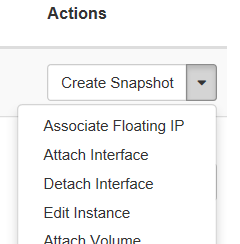
\includegraphics[scale=0.7]{img/associate_IP_1.png}
\end{center}
\item A pop-up window will appear and under IP Address select from the
  drop-down menu an IP address from the available pool.
\begin{center}
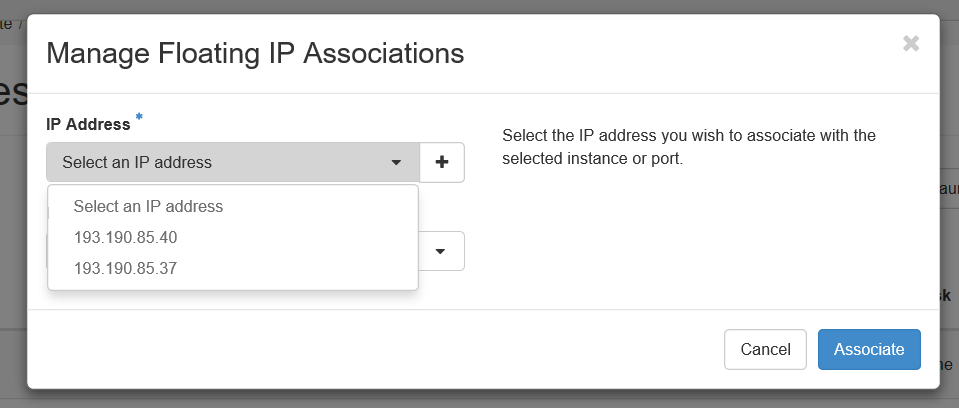
\includegraphics[scale=0.5]{img/associate_IP_2.png}
\end{center}
\item Click Associate
\end{enumerate}

If the IP has been successfully associated in the upper right corner of the browser screen will appear a green confirmation. If not successful a red notification will pop up that something went wrong.

\strong{Note:} To disassociate an IP address from an instance, click
the Disassociate button in the Actions column.

% TODO: remove this warning once we've removed the "Release Floating
% IP" buttons from the dashboard.
\strong{Warning:} \emph{Do not} use the Release Floating IP option in
the Actions column or on the overview page.  This will remove the
floating IP from the pool assigned to your project, something which
you, as a regular user, cannot undo.  If you've accidentally released
a floating IP, contact \cloudinfo to have it restored.

%%% Local Variables:
%%% mode: latex
%%% TeX-master: "intro-OpenStack"
%%% End:
